\clearpage
\chapter[IMPLEMENTATION AND EXPERIMENTAL WORK]{Implementation and Experimental Work}
\label{ch:impl}

\section{Implementation Environment}
\begin{table}[!htbp]
\centering
\caption{Implementation environment.}
\label{tab:env}
\small
\renewcommand{\arraystretch}{1.2}
\begin{tabularx}{\textwidth}{>{\raggedright\arraybackslash}p{4.2cm}>{\raggedright\arraybackslash}X}
\toprule
\textbf{Part} & \textbf{Technology}\\
\midrule
Language and runtime & TypeScript on Node.js 22 (server run with \texttt{tsx}); a small amount of JavaScript in the traffic generator; optional Python~3\\
Server & Express~5, \texttt{ws} for WebSocket, \texttt{ssh2} for SSH (no \texttt{ssh} binary needed)\\
Dashboard & React~19, Vite~8, \texttt{@xyflow/react} for the 2D graph, Three.js with react-three-fiber for the 3D scene, Recharts, Framer Motion\\
Persistence & JSON files under \texttt{server/data} (graph state, remote configuration, per-target connection events); metric ring buffers in memory\\
Source size & About 18\,400 lines of TypeScript in the server and 17\,200 in the dashboard; 5\,400 in the evaluation tools; 2\,500 in the \texttt{v2} studies\\
Tests & 339 automated tests in 19 suites, run with Node's built-in test runner\\
Version control & Git, with GitHub as the remote\\
\bottomrule
\end{tabularx}
\end{table}

\section{Module-wise Implementation}

\subsection{Connection and collection}
The connection manager keeps one SSH session per target and runs commands from a fixed catalogue. The catalogue is a list of command builders; every argument that reaches a shell is sanitised (container identifiers must match the shapes Docker itself produces, timestamps and tail lengths are validated). Timeouts are sized for a loaded host: on a swap-thrashing 2\,GB machine with eighteen JVM services, \code{docker ps} was measured at 45 seconds, and a timeout shorter than that does not degrade gracefully, it makes the whole target disappear from the graph.

Each cycle the collector asks for the container list, inspects containers it has not seen, reads statistics, and reads each container's socket table. Reading the table through the container's process id on the host (\code{/proc/<pid>/net/tcp}) works for every image, including images with no shell, which had silently hidden the front end of one benchmark for weeks before it was changed. The same command returns the interface byte counters, which are exact, where \code{docker stats} prints values rounded to three significant figures.

\subsection{Edge direction, weights and the graph}
Every connection appears in the socket tables of both ends. Recording ``scanned container calls peer'' on both sides produced a reverse duplicate for every real link, so the graph was effectively undirected: it put a cycle on every pair, which made ``downstream of X'' reach almost the whole graph and made blast radius and criticality saturate. Direction is now recovered from listening ports: whichever end owns the listening port is the callee. The ephemeral port range is a fallback when a container's listen table could not be read, and when neither settles it the edge is marked unresolved instead of being given a coin flip dressed as a measurement.

Observed and declared edges are merged, and an observed edge expires ten minutes after it was last seen. A connection that is seen only as a recently closed socket (TIME\_WAIT, which lingers about a minute) is counted once by its connection key, so a burst of short calls does not look like many links. A call made through the host's address to a port that one service publishes is attributed to that service (a connection to a private or bridge-gateway address on a published port).

\subsection{Container facts}
The container runtime's state is turned into one of a few facts: down (exited with a non-zero code, dead or vanished), paused, restarting, or detached from its network while running; repeated restarts in a short window are flagged separately as a crash loop. A load generator and a container that finished cleanly are \emph{benign}: traffic is started and stopped by people, not by faults.

\subsection{The load factor and the load-aware level}
Listing~\ref{lst:loadfactor} reads the project's load and the slope of each signal on it: the median shift of the signals that carry traffic, and a ridge estimate pulled towards the prior. Listing~\ref{lst:judge} is the judgement of one reading: a signal is tried under both hypotheses about how it follows the load, and counts as unusual only if neither explains it; the strongest signal sets the service's level and is kept as the evidence.

\lstinputlisting[language=TS,caption={The load factor and its slopes (loadModel.ts).},label={lst:loadfactor}]{listings/load_factor.ts}
\lstinputlisting[language=TS,caption={Judging a reading against what the load predicts (loadModel.ts).},label={lst:judge}]{listings/load_level.ts}

\subsection{Ranking by random walk}
Listing~\ref{lst:walk} is the personalised random walk. The ``stay'' weight is what lets the true source keep the walker: a service whose trouble nothing downstream explains collects the most time.

\lstinputlisting[language=TS,caption={Root cause by random walk (randomWalk.ts).},label={lst:walk}]{listings/walk.ts}

\subsection{Learned propagation}
The cascade model has two halves (Algorithm~\ref{alg:cascade}): counting trials and successes per edge while the system runs, and spreading risk up the graph by noisy-OR from the suspected root when an incident is open.

\subsection{Hybrid fusion and the three engines in parallel}
Listing~\ref{lst:fuse} is the fusion of rules and ML. The default detection mode is \texttt{or-strict}: the alarm value is the larger of the ML level and the rule score divided by 1.25. On every cycle the incident manager records the verdict of each engine (alarm, peak against its own line, top five suspects) whichever one is active, and keeps the last 90 peaks for the Detection engines page; only the active engine opens and closes incidents.

\lstinputlisting[language=TS,caption={Fusing rules and ML (hybrid.ts).},label={lst:fuse}]{listings/fuse.ts}

\subsection{Incidents}
The incident manager, once per target per cycle, runs the three engines' shared step, builds the evidence for the active engine, calls the root-cause engine, and either updates the open incident or opens a new one. A new incident takes the status \texttt{DEGRADED} or \texttt{INCIDENT} according to whether any service is critical; it is resolved when the alarm clears and stays in the history. Severity is raised when more than a configured number of services are critical, and lowered for a service that nothing depends on and that depends on nothing, which has no blast radius.

\subsection{Traffic generation}
The traffic controller starts and stops load through the traffic generator's HTTP API. Each application has a workflow file (a set of weighted user journeys with think times) and a set of profiles (baseline, moderate, heavy, stress, ramp) that fix the number of virtual users and their pace. An application that has no file of its own gets a generic front-page workflow; before that change the server refused every project outside five named ones with ``no workflow defined''.

\section{Algorithms}
Algorithm~\ref{alg:window} is one decision window and Algorithm~\ref{alg:cascade} the learning and prediction step of the cascade model.

\begin{algorithm}[!htbp]
\caption{One decision window of the diagnosis assistant}
\label{alg:window}
\begin{algorithmic}[1]
\Require readings $x_s(t)$, container states, graph $G$ with learned directions
\Ensure alarm, ranked causes, likely-next set, fault type, runbook
\State \textbf{facts}: mark each service stopped, paused, restarting, detached or crash-looping
\State \textbf{score}: model levels $\lambda_s$ (own and symptom), rule scores $\rho_s$, anomalies $a_s$
\State \textbf{alarm}: apply the hybrid rule; if no alarm, update the propagation counts and stop
\State \textbf{rank}: services with a fact first, then by the walk share $\pi_s$ over $G$
\State \textbf{explain}: report own versus symptom evidence and what the neighbours explain
\State \textbf{predict}: $P(c)$ by Eq.~\eqref{eq:noisyor} from the top suspect; early-warning flags
\State \textbf{diagnose}: classify the fault type of the top suspect; attach its runbook
\State update $\hat p(c \leftarrow x)$ from services that newly turned abnormal
\end{algorithmic}
\end{algorithm}

\begin{algorithm}[!htbp]
\caption{Learning propagation and predicting the next services}
\label{alg:cascade}
\begin{algorithmic}[1]
\Require set of services newly abnormal $O$, set of abnormal services $A$, call graph
\Ensure edge probabilities $\hat p$; risk $P(c)$ for healthy services
\For{each open trial $(c, x)$}
  \If{$c \in A$} record a success \ElsIf{the window of 12 steps ran out} record a failure \EndIf
\EndFor
\For{each $x \in O$ and each healthy caller $c$ of $x$} open the trial $(c,x)$ \EndFor
\State $\hat p(c \leftarrow x) \gets (k + m\pi_0)/(n + m)$ for every edge
\State for a suspected root $r$: $P(r) = 1$; sweep the callers upwards, $P(c) = 1 - \prod_{x \in C(c)} (1 - P(x)\hat p(c \leftarrow x))$
\State drop services that are already abnormal; report the rest above the risk cut
\end{algorithmic}
\end{algorithm}

\section{Application Programming Interfaces}
The server exposes 64 REST endpoints and one WebSocket. They fall into ten areas: the graph (topology, node detail and metric history), targets (registered hosts and their discovery), reliability (cascade risk, what-if failure, blast radius), incidents (list, evidence, propagation, timeline), engines (active engine, per-engine verdicts, the switch), traffic (start, stop, status, entry points), experiments, the optional ML sidecar, configuration (hosts, keys, reset) and ingest (push from the optional standalone collector). The WebSocket carries \texttt{graph-update} (nodes, edges, targets, every 5 seconds), \texttt{incident.updated}, \texttt{trace-events} (the live connection feed) and the embedded terminal's data, so the dashboard does no polling for graph state.

\section{Configuration and Deployment}
\begin{sloppypar}
The server is configured by a few environment variables: \texttt{PORT} (3001), \texttt{POLLING\_INTERVAL\_MS} (5000), \texttt{METRIC\_HISTORY\_SIZE} (720 readings, one hour), \texttt{INGEST\_TOKEN} (to be changed when the server is reachable by others), \texttt{MAPPER\_ENGINE} (engine at start), \texttt{MAPPER\_BASELINE\_MIN} (30 minutes of baseline before a project's learned rule model is used) and \texttt{MAPPER\_AUTO\_RESTART} (\texttt{off} stops the mapper restarting crashed containers).
\end{sloppypar}

A host is added in the dashboard with its address, SSH user and key path. The configuration is saved to \texttt{server/data/remote\_config.json}; private keys are never copied into the repository, and \texttt{*.pem} is git-ignored as a backstop. \texttt{npm start} installs what is missing and starts the server and the dashboard; \texttt{npm run doctor} checks the machine; \texttt{npm run hosts} lists hosts and tests port 22; \texttt{npm run check-host} and \texttt{npm run mapper-edges} diagnose a host and what the mapper holds for it (Section~\ref{sec:tools}).

\begin{table}[!htbp]
\centering
\caption{Engine parameters (defaults).}
\label{tab:params}
\small
\renewcommand{\arraystretch}{1.2}
\begin{tabularx}{\textwidth}{>{\raggedright\arraybackslash}p{5.2cm}>{\raggedright\arraybackslash}p{2.2cm}>{\raggedright\arraybackslash}X}
\toprule
\textbf{Parameter} & \textbf{Value} & \textbf{Meaning}\\
\midrule
Training window & 120 readings & About ten minutes of normal behaviour\\
Slow reference & 360 readings & Median that shifts are measured from (half an hour)\\
Readings before judging & 30 & First baseline\\
Baseline refresh & every 4 readings & Median and spread per signal and hypothesis\\
Signal units $u_f$ & CPU 5, memory 1, network 2000, requests 0.1 & Below about one unit a change is noise\\
Carrying signal & 0.4 above idle & A signal that says something about the load\\
Slope prior / ridge weight & 1 (network, requests), 0.4 (CPU) / 60 & Load response before any load change has been seen\\
Alarm line $z_{\mathrm{line}}$ & 4 robust spreads & Level 1; spread is the larger of MAD and the 90th-percentile distance\\
Alarm level / persistence & 2 / 2 windows & Model condition of the hybrid alarm\\
Rules alone trusted at & 1.25 $\times$ line & Rule condition of the hybrid alarm\\
Drift & 24 or 360 readings & Mild shift accepted in two minutes; large one quarantined for thirty\\
Walk restart / iterations & 0.15 / 60 & Random walk\\
Propagation trial window & 12 windows & One minute\\
Propagation prior & mean 0.5, weight 2 & Uninformative\\
Forecast window / horizon / $R^2$ & 24 / 24 / 0.6 & Two minutes fitted, two minutes ahead\\
\bottomrule
\end{tabularx}
\end{table}

\section{Experimental Setup and Test Cases}
The experiments run on the two benches of Section~\ref{sec:benches} (ShopFlow, 13 services, and LedgerLine, 12, for 217 minutes each with open-loop traffic and 62 blind faults), on a synthetic tuning split (16 campaigns, 170 faults, seed 1) and a disjoint test split scored once (16 campaigns, 178 faults, seed 2), with a 5-second collection period; Section~\ref{sec:evaldesign} gives the design. Intervals are 95\% percentile bootstrap, and engine contrasts use the paired bootstrap. The test cases that hold the implementation are described in Section~\ref{sec:testing}.

\section{Prototype and System Implementation}
\label{sec:prototype}
The figures below are screenshots of the running dashboard. The 2D pages and the Detection engines page were taken on the shop that the ground-truth simulator drives (10 services, 9 edges), so that the same data could be shown with and without a fault; the 3D views were taken on the live ShopFlow bench.

\subsection{Architecture view}
The 2D view draws the dependency graph with a choice of arrangements (clusters, hierarchy, tiers, grid, circle, polygon, radial, spiral) and filters by service type. Nodes show CPU and memory against the container's own allowance; edges show the dependency and, when observed, its activity.

\begin{figure}[!htbp]
\centering
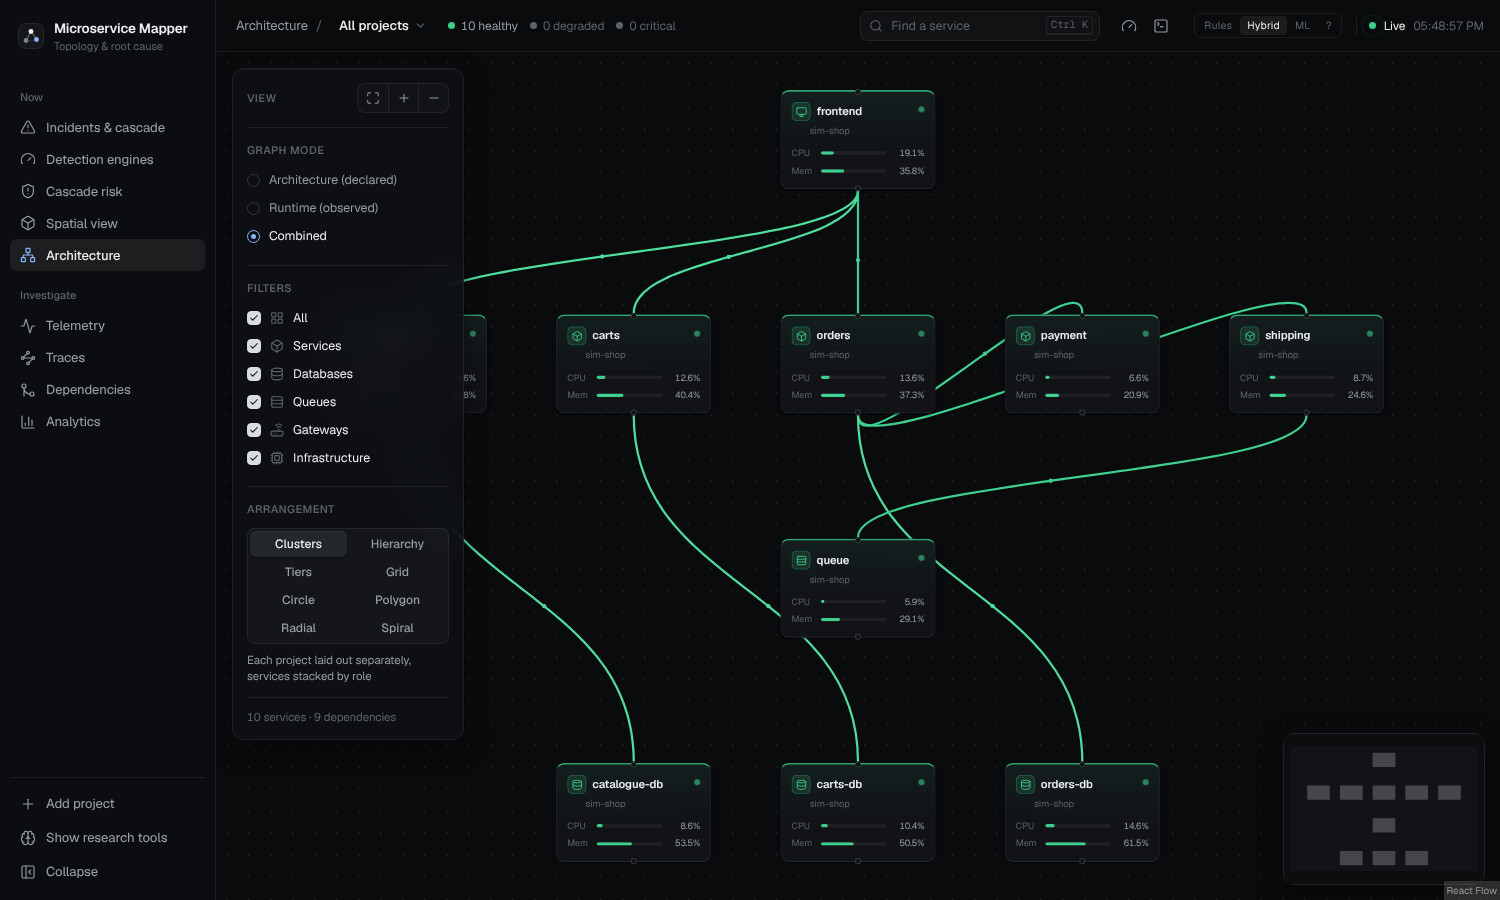
\includegraphics[width=\textwidth]{ui_architecture.jpg}
\caption{Architecture view: the dependency graph of the simulated shop, with arrangement and filter controls.}
\label{fig:ui-arch}
\end{figure}

\subsection{Incidents and cascade}
When the alarm is raised the page shows the most likely root cause, the confidence, the severity and the number of affected services. Below it, the cascade panel shows the source, the services already affected (observed) and those next in line (predicted); the ranking lists each service with the strongest signal behind its score; the ``Why'' panel splits a score into its own-level, symptom-level and walk components and lists the evidence that raised it; and the next steps give concrete commands for the host.

\begin{figure}[!htbp]
\centering
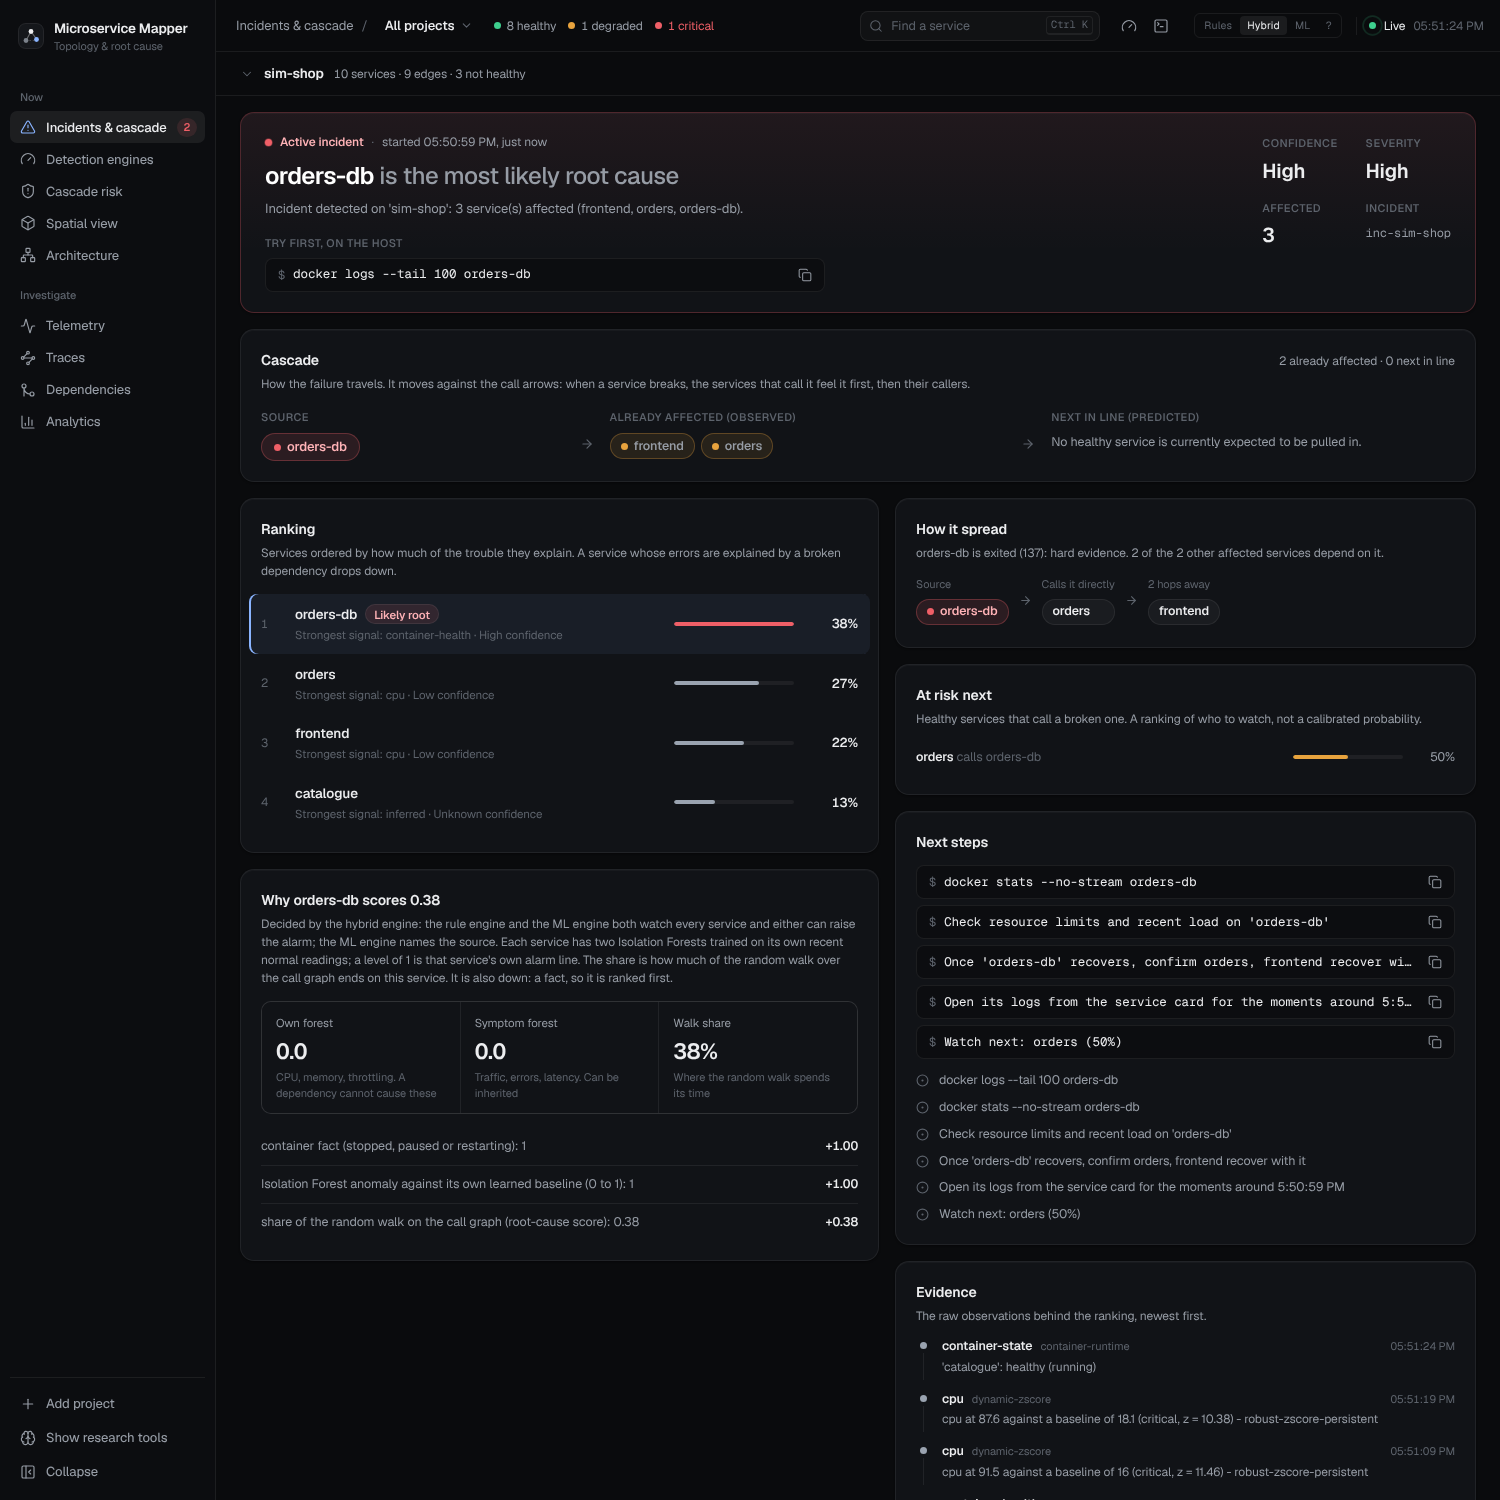
\includegraphics[width=\textwidth]{ui_incident_active.png}
\caption{An active incident after \texttt{orders-db} was killed: root cause, cascade, ranking, evidence breakdown and next steps.}
\label{fig:ui-incident}
\end{figure}

\subsection{Detection engines}
The Detection engines page (Figure~\ref{fig:ui-engines-alarm}) is where a developer checks what the engine switch actually changes. The top half explains the three engines in four short lines each (what decides, how the source is named, the strength, the weakness) and states the Hybrid rule as a formula. Below it the three engines run side by side on the same readings, every cycle, whichever one is active. Each column names its top suspect, and the ML column also says \emph{why}: in Figure~\ref{fig:ui-engines-alarm} it reads ``payment, cpu 10.3 spreads from what the load predicts''. A small chip next to the project name says whether the shared workload moved (``workload steady'' or ``traffic $\times$2.4, explained, not a fault''), so a user can see at a glance that a traffic swing was taken out before any service was judged.

Under the columns are six charts: each engine's peak against its alarm line, a strip showing on which cycles the engines agreed, the level of every service under every engine, a source-or-victim scatter (own resources against symptoms), the share of blame from the random walk, and a trail for one chosen service. Every chart has an enlarge button; the enlarged view (Figure~\ref{fig:ui-engines-popup}) adds a time brush so a stretch of a few cycles can be zoomed into, and closes with Esc. The page ends with the configuration of both engines in plain words.

\begin{figure}[p]
\centering
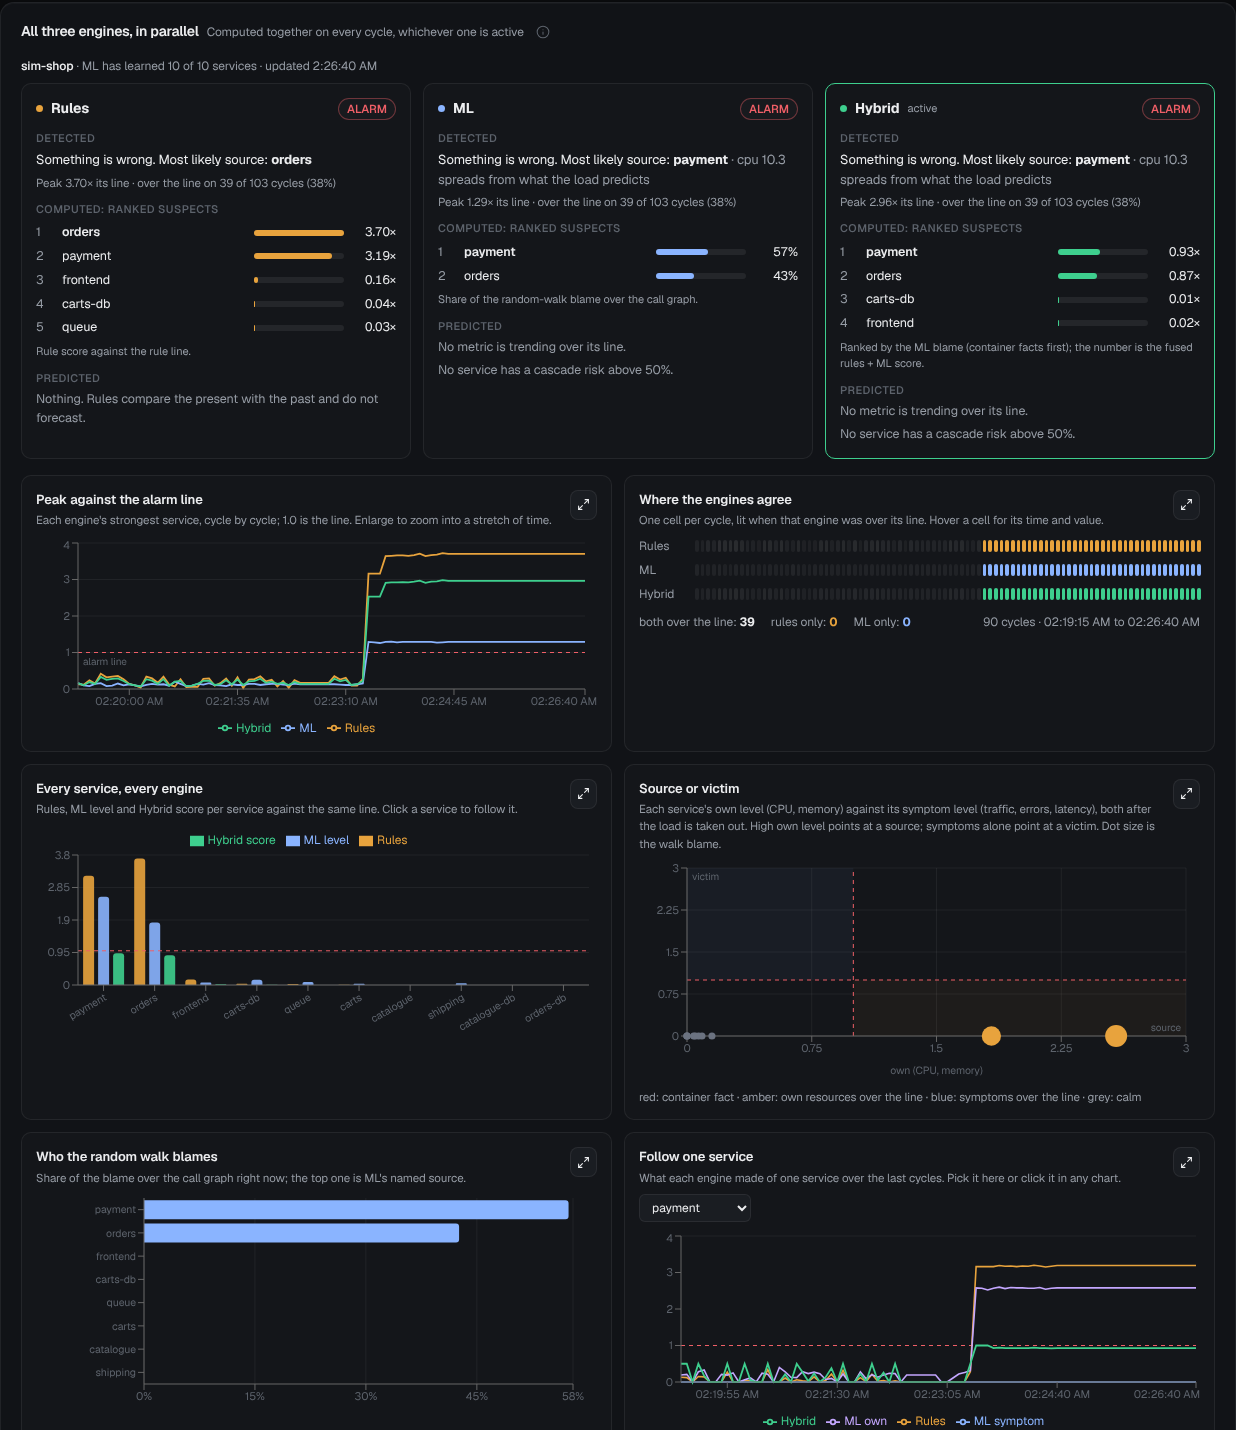
\includegraphics[width=0.96\textwidth,height=0.82\textheight,keepaspectratio]{ui_engines_alarm.png}
\caption[The Detection engines page during a slow-payment fault]{The parallel view during a slow-payment fault. Rules blame \texttt{orders} (the louder victim); ML and Hybrid name \texttt{payment} and say which signal moved. Below: peak against the line, agreement strip, every service, source or victim, walk blame and one service's trail.}
\label{fig:ui-engines-alarm}
\end{figure}

\begin{figure}[!htbp]
\centering
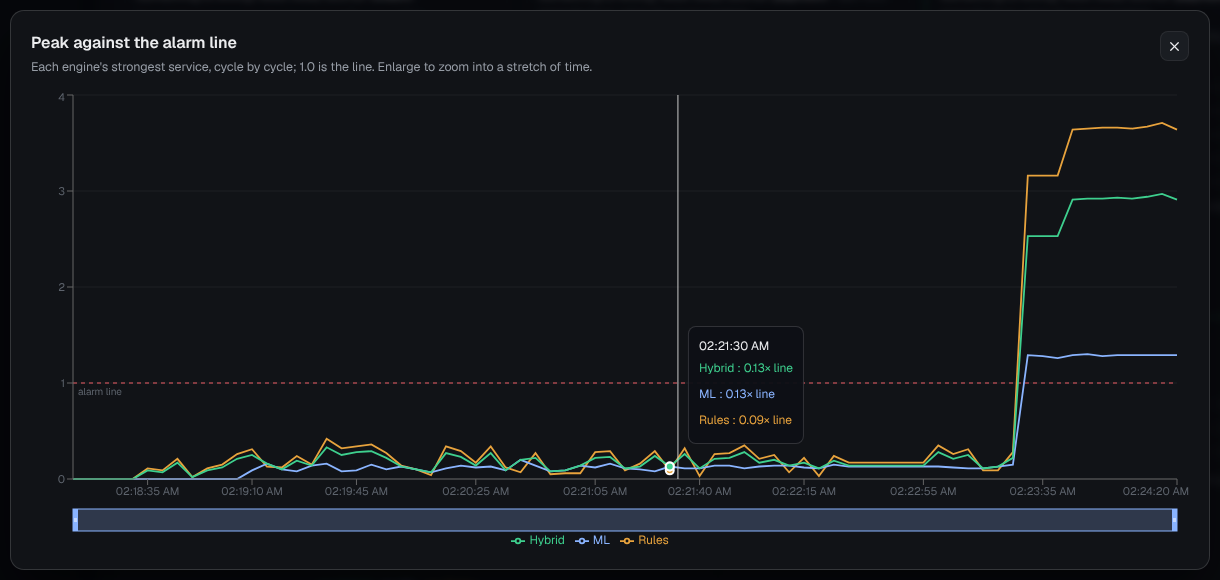
\includegraphics[width=0.82\textwidth]{ui_engines_popup.png}
\caption[An enlarged engine chart with its time brush]{An enlarged chart with its time brush and hover read-out. The ML peak crosses the line once and stays just above it; the rule score climbs higher but on the wrong service.}
\label{fig:ui-engines-popup}
\end{figure}

\subsection{Cascade risk}
The cascade-risk page shows what is failing now and on its own measurements, what is exposed, and what would happen if a chosen service failed (what-if), with the model's name and parameter beside every prediction rather than a bare number.

\begin{figure}[!htbp]
\centering
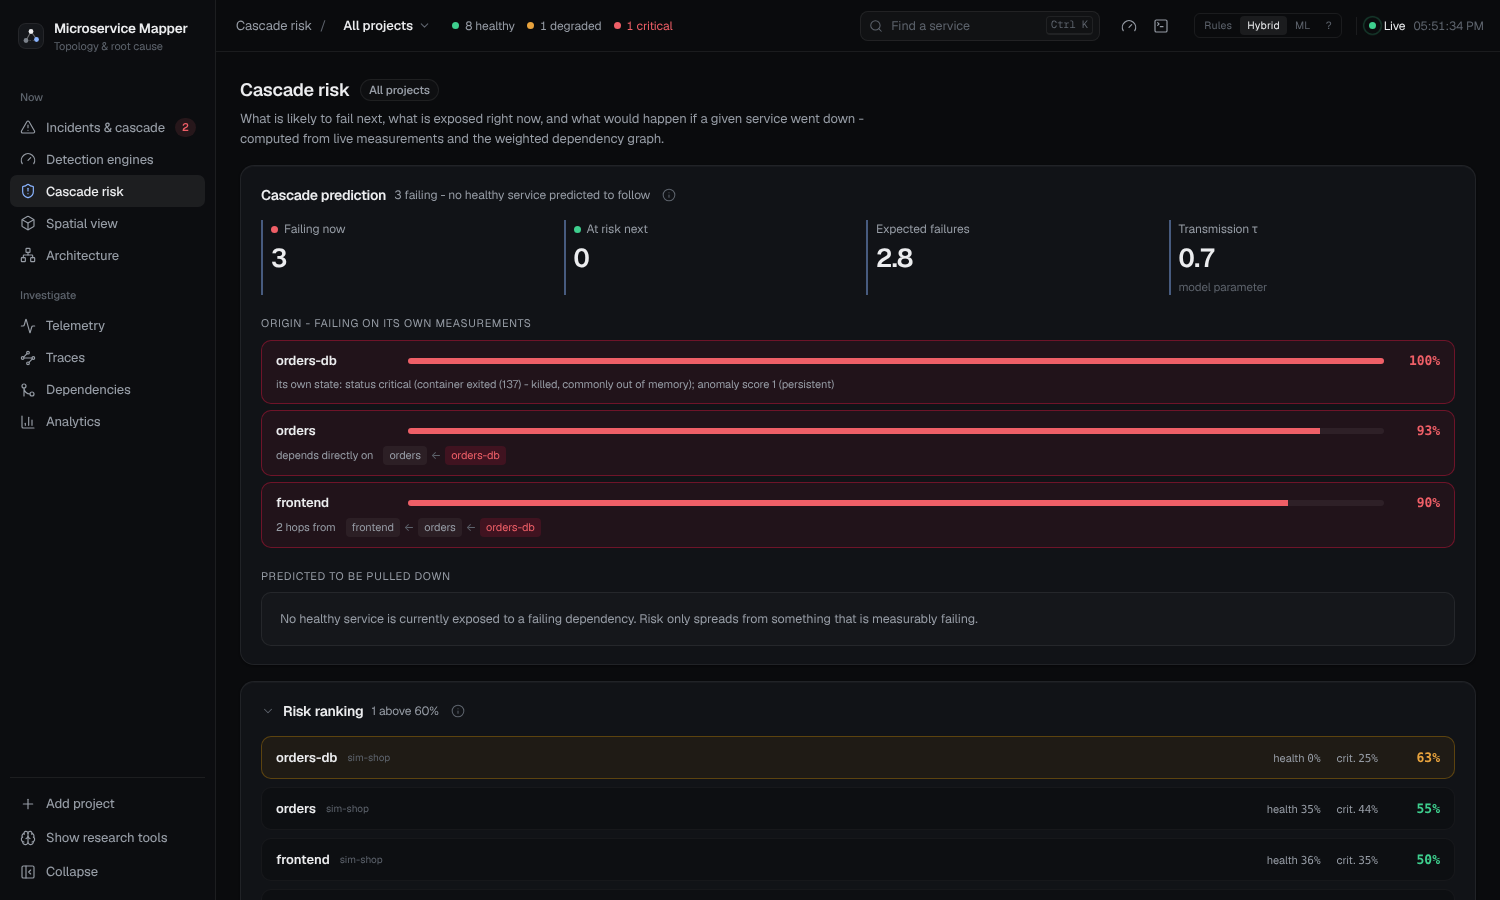
\includegraphics[width=\textwidth]{ui_cascade_risk_fault.png}
\caption{Cascade risk during the fault: the origin and the services failing on their own measurements, expected failures and transmission.}
\label{fig:ui-cascade}
\end{figure}

\subsection{Telemetry, traces, dependencies and analytics}
Four pages support the investigation (Figure~\ref{fig:ui-pages}). Telemetry shows fleet totals, the live connection log and a sortable per-service table with a history chart. Traces shows connection tracing as a ring, a matrix and an event stream; these are sampled TCP sockets, not requests. Dependencies lists every connection with its declared and observed flags and its evidence sources. Analytics gives a health index, the counts of healthy, degraded and critical services, the most connected services and the top CPU and memory users.

\begin{figure}[!htbp]
\centering
\setlength{\tabcolsep}{2pt}
\begin{tabular}{cc}
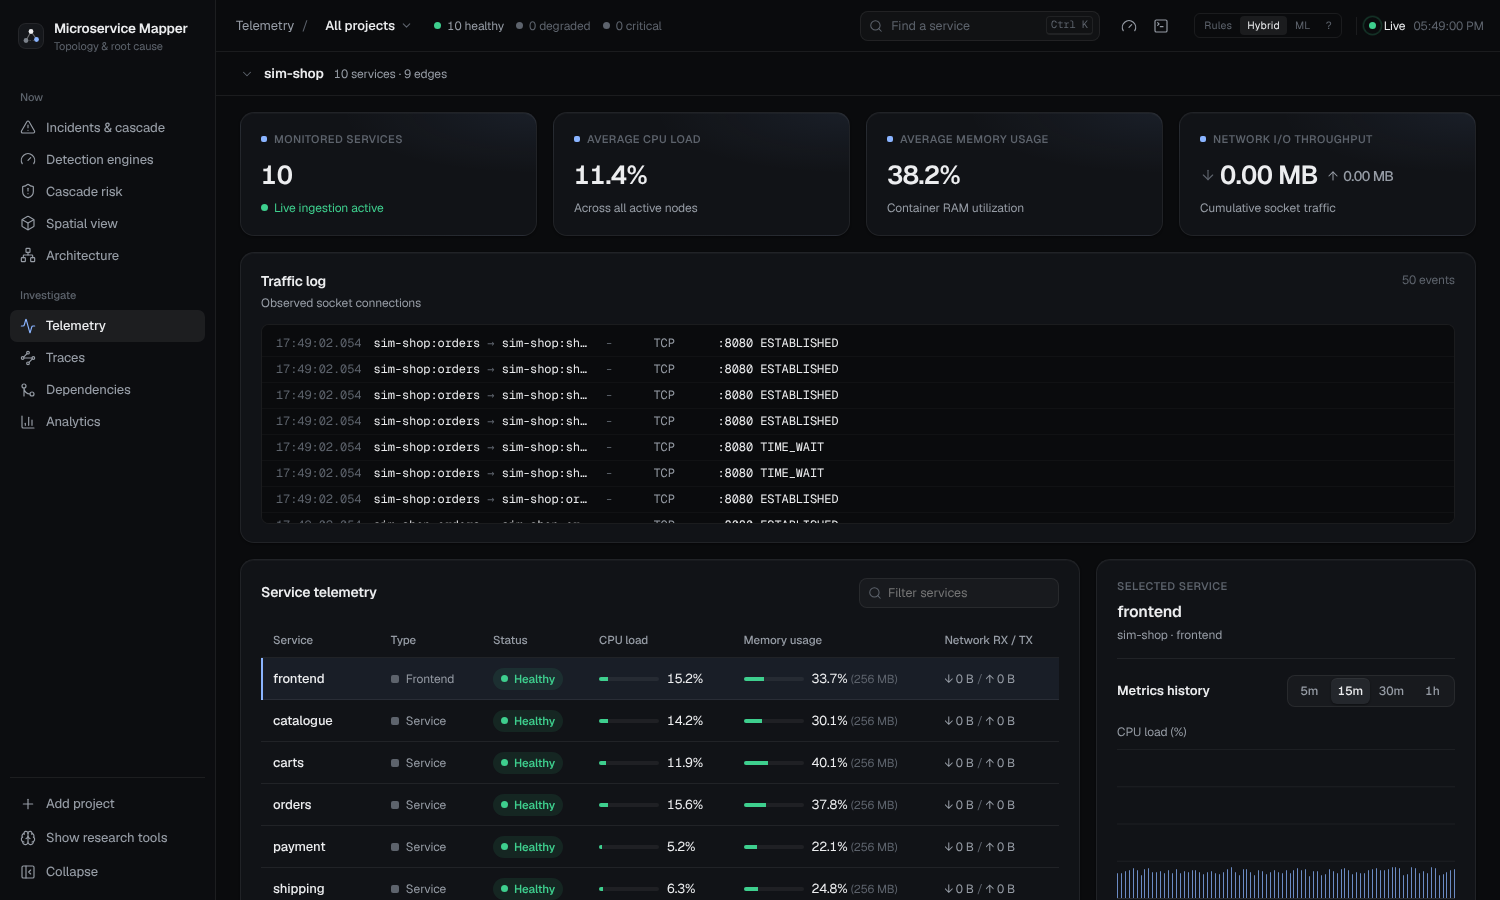
\includegraphics[width=0.49\textwidth]{ui_telemetry.png} & 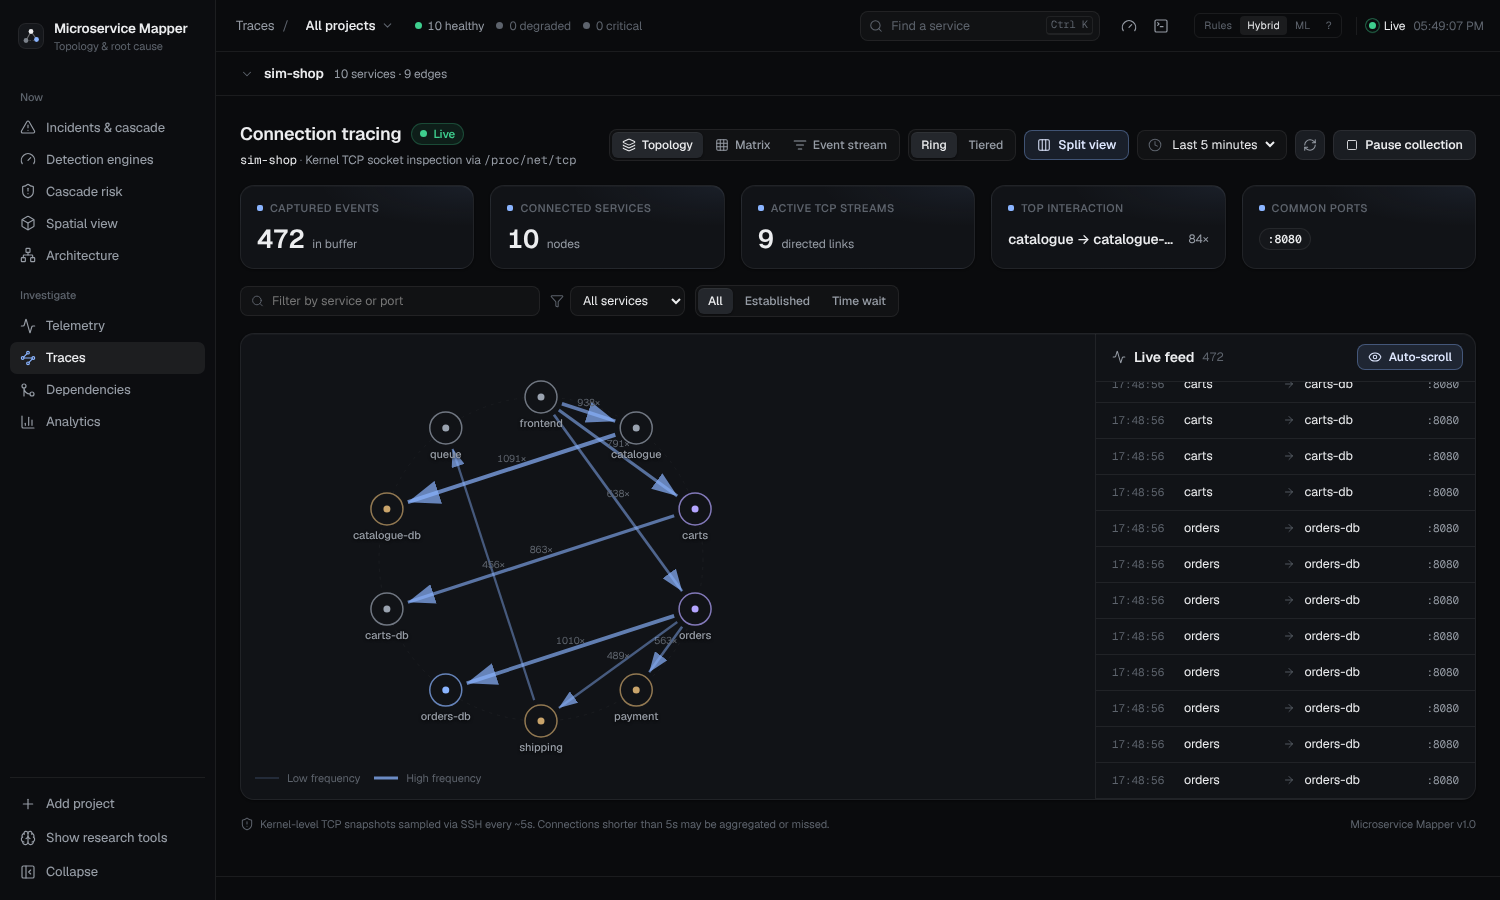
\includegraphics[width=0.49\textwidth]{ui_traces.png}\\
\small (a) Telemetry & \small (b) Traces\\[4pt]
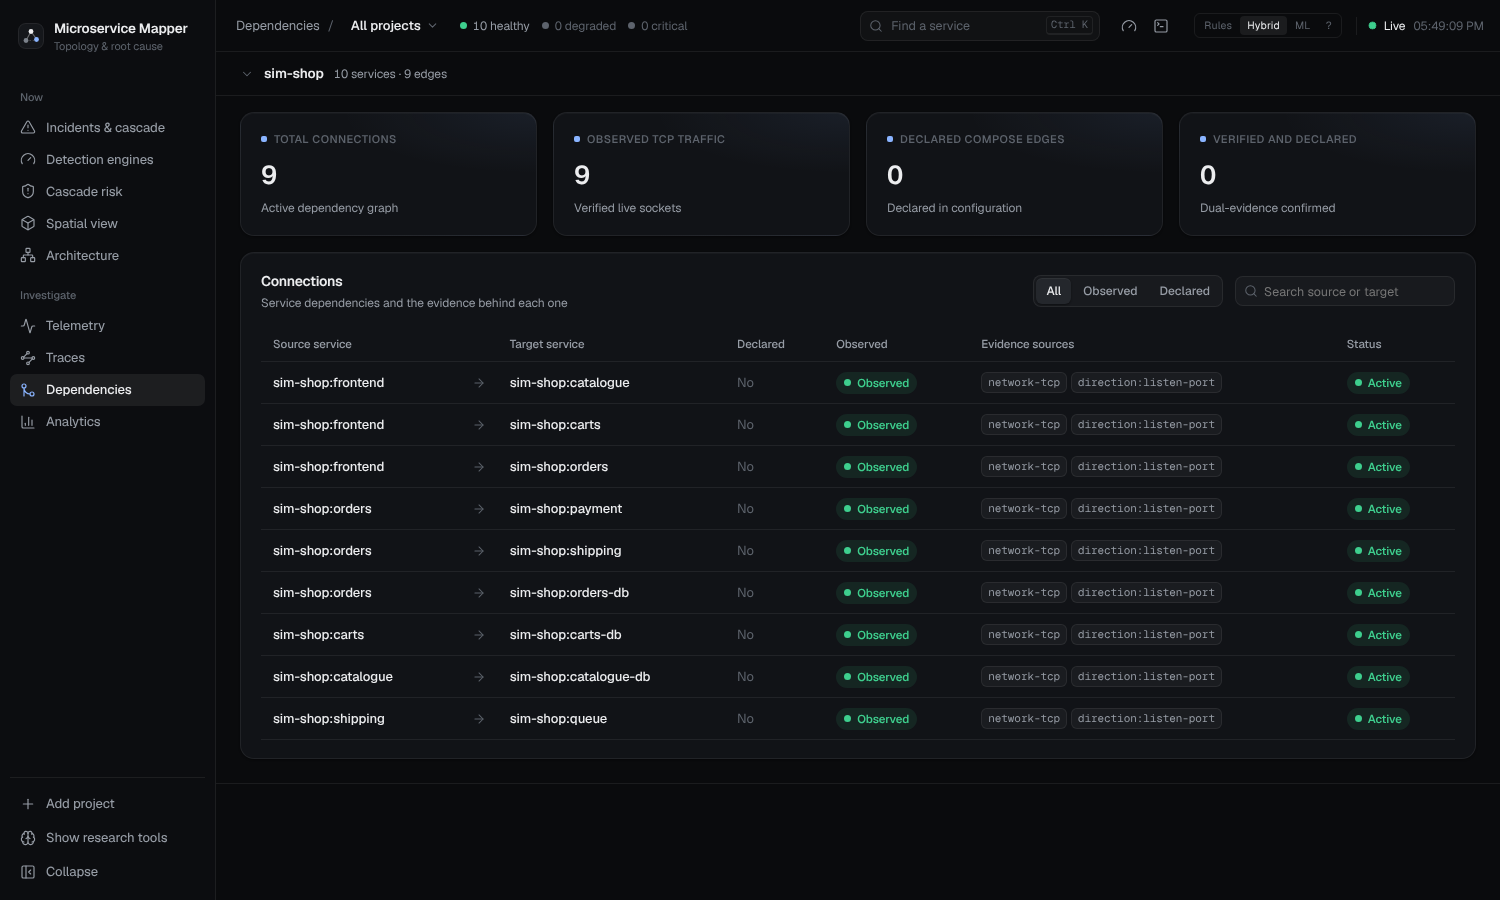
\includegraphics[width=0.49\textwidth]{ui_dependencies.png} & 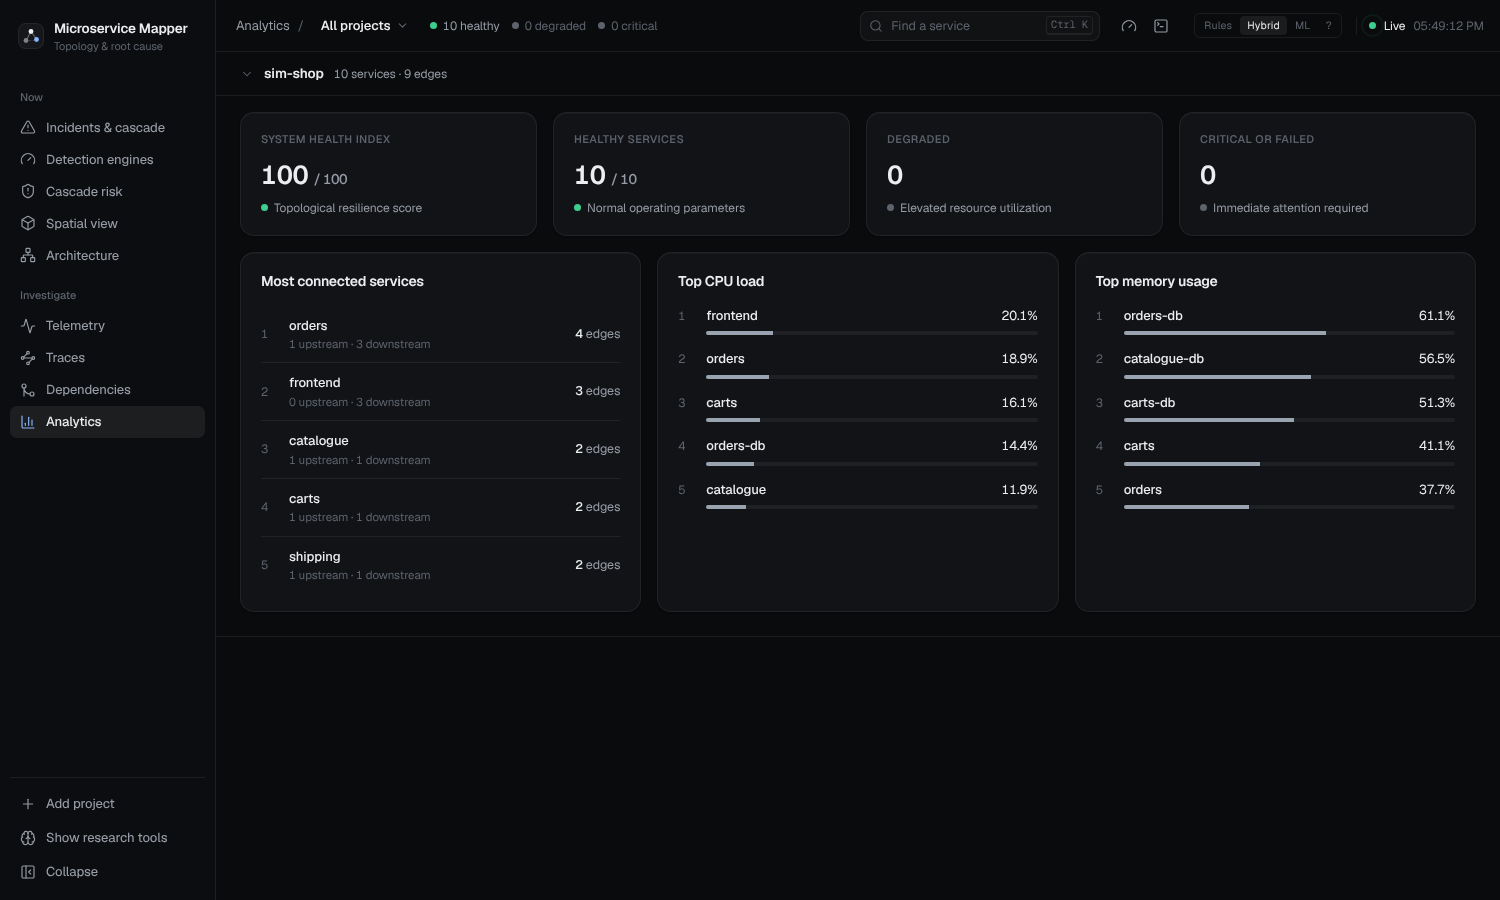
\includegraphics[width=0.49\textwidth]{ui_analytics.png}\\
\small (c) Dependencies & \small (d) Analytics
\end{tabular}
\caption[The telemetry, traces, dependencies and analytics pages]{The investigation pages: (a) telemetry with fleet totals and a per-service table, (b) connection traces as ring, matrix and event stream, (c) dependencies with their evidence (here \emph{network-tcp} and \emph{direction:listen-port}), (d) analytics.}
\label{fig:ui-pages}
\end{figure}

\subsection{The 3D spatial view}
The 3D scene shows the same graph as a small city, and each arrangement answers a different question a developer asks while debugging. Services are units on platforms; links are cables whose thickness shows the dependency weight and whose colour shows the heat of the link, with pulses that move at a rate driven by the link's request rate. A floating card over each platform gives its role, how many services it holds and their state. The figures were taken on the live ShopFlow bench, with the scene focused on that project.
\begin{itemize}
\item \textbf{Islands} (Figure~\ref{fig:3d-islands}) groups services by role: edge, services, messaging and data, each on its own raised platform.
\item \textbf{Flow} (Figure~\ref{fig:3d-views}a) lays the platforms out in the order a request travels: the entry points, then the services one hop away, two hops away and so on. Each card says how many callers a fault at that hop can reach, so the platform to look at first is the one whose card says the most.
\item \textbf{Topology} (Figure~\ref{fig:3d-views}b) sorts services by how much depends on them: the most depended-on, the depended-on, and those nothing depends on. It is the blast-radius view: a fault on the first platform hurts the most.
\item \textbf{Tiers} (Figure~\ref{fig:3d-views}c) stacks the architectural layers as terraces from edge (L4) down to data (L1), with the calls in and out of each layer on its card, so a call that skips a layer or goes up the stack stands out.
\end{itemize}
During a fault the failing unit is boxed in red with a callout naming it and its score, its platform is tinted, the card changes from ``all healthy'' to the count of degraded services, and the bell in the corner counts what needs attention (Figure~\ref{fig:3d-islands}b).

\begin{figure}[!htbp]
\centering
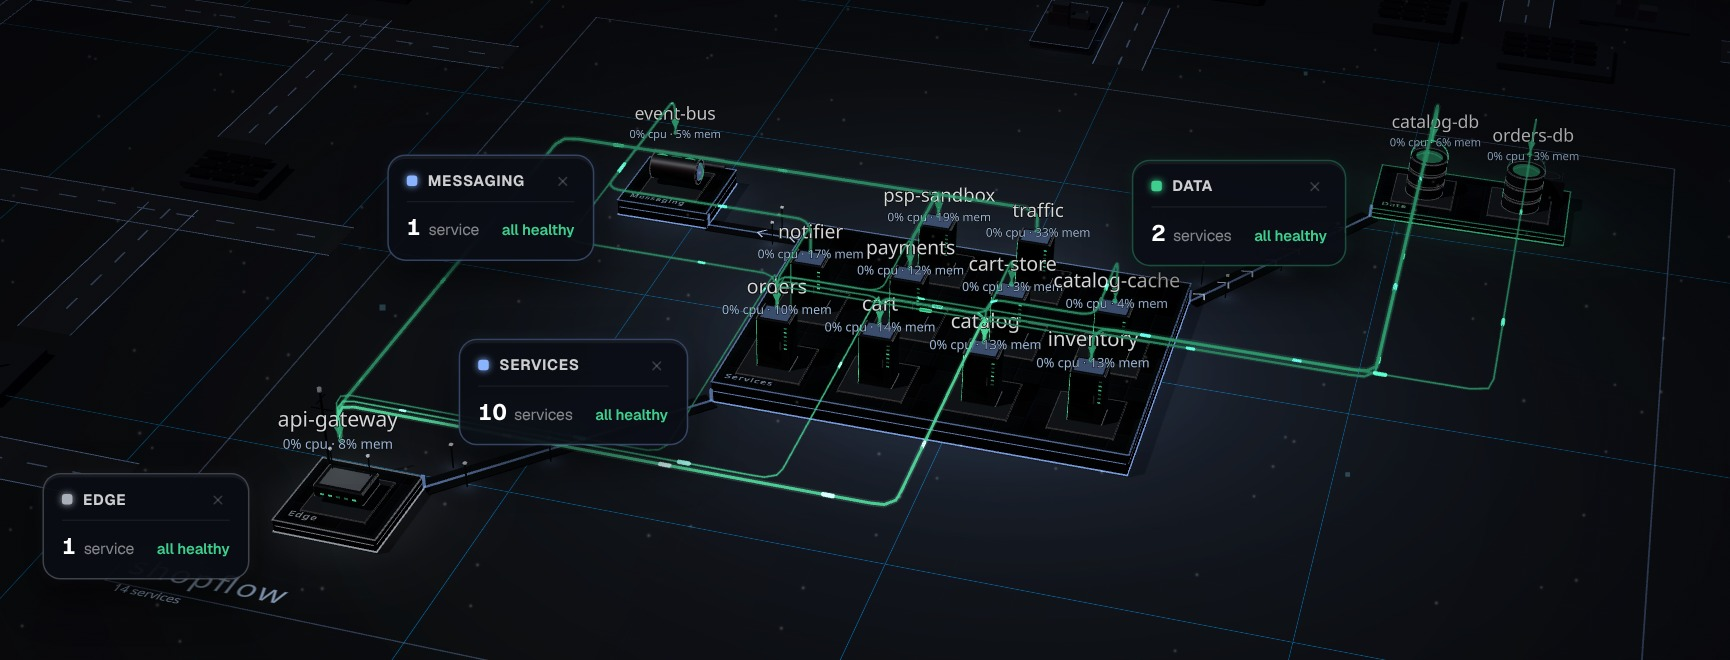
\includegraphics[width=\textwidth]{ui3d_islands.jpg}\\[-1pt]
{\small (a) Healthy}\\[6pt]
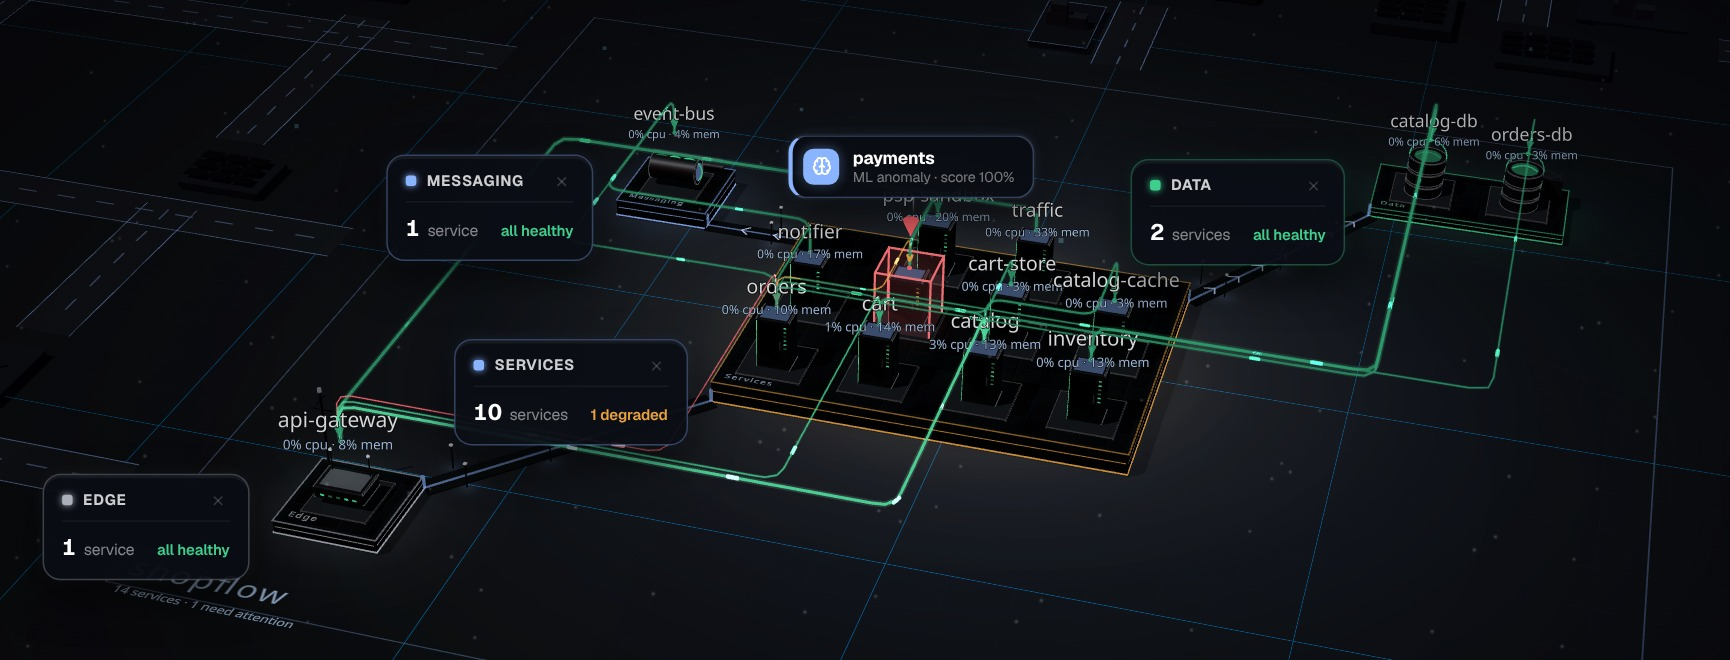
\includegraphics[width=\textwidth]{ui3d_islands_fault.jpg}\\[-1pt]
{\small (b) During a fault: \texttt{payments} paused}
\caption[The 3D Islands view of the ShopFlow bench, healthy and during a fault]{The 3D Islands view of the live ShopFlow bench: one platform per role with a card giving its size and state. (b) The same view with \texttt{payments} paused: the unit is boxed in red, its platform tinted and its card updated.}
\label{fig:3d-islands}
\end{figure}

\begin{figure}[p]
\centering
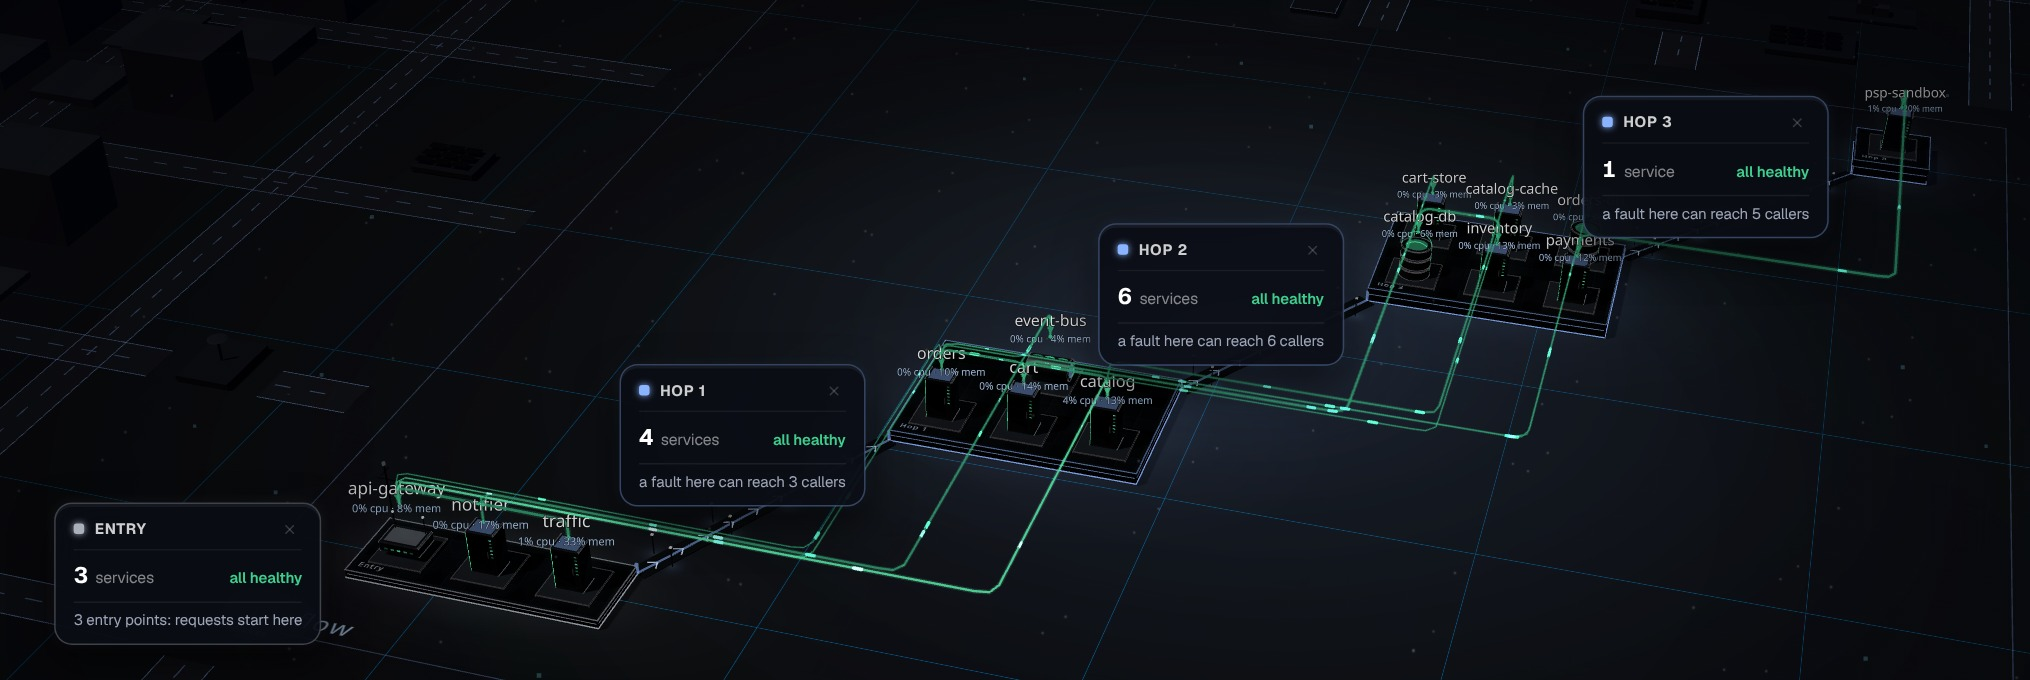
\includegraphics[width=\textwidth]{ui3d_flow.jpg}\\[-1pt]
{\small (a) Flow: the request path, hop by hop}\\[6pt]
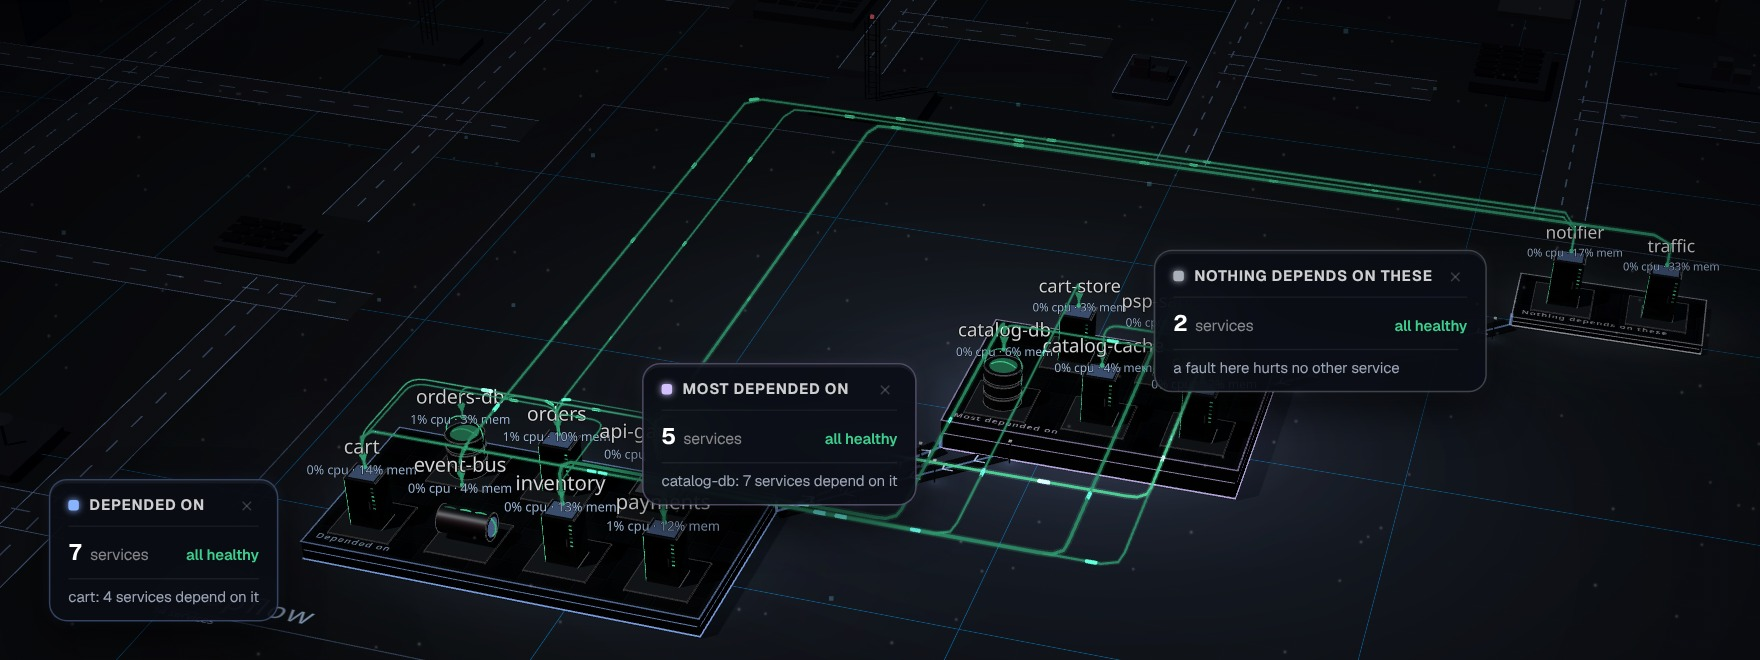
\includegraphics[width=\textwidth]{ui3d_topology.jpg}\\[-1pt]
{\small (b) Topology: by how much depends on each service}\\[6pt]
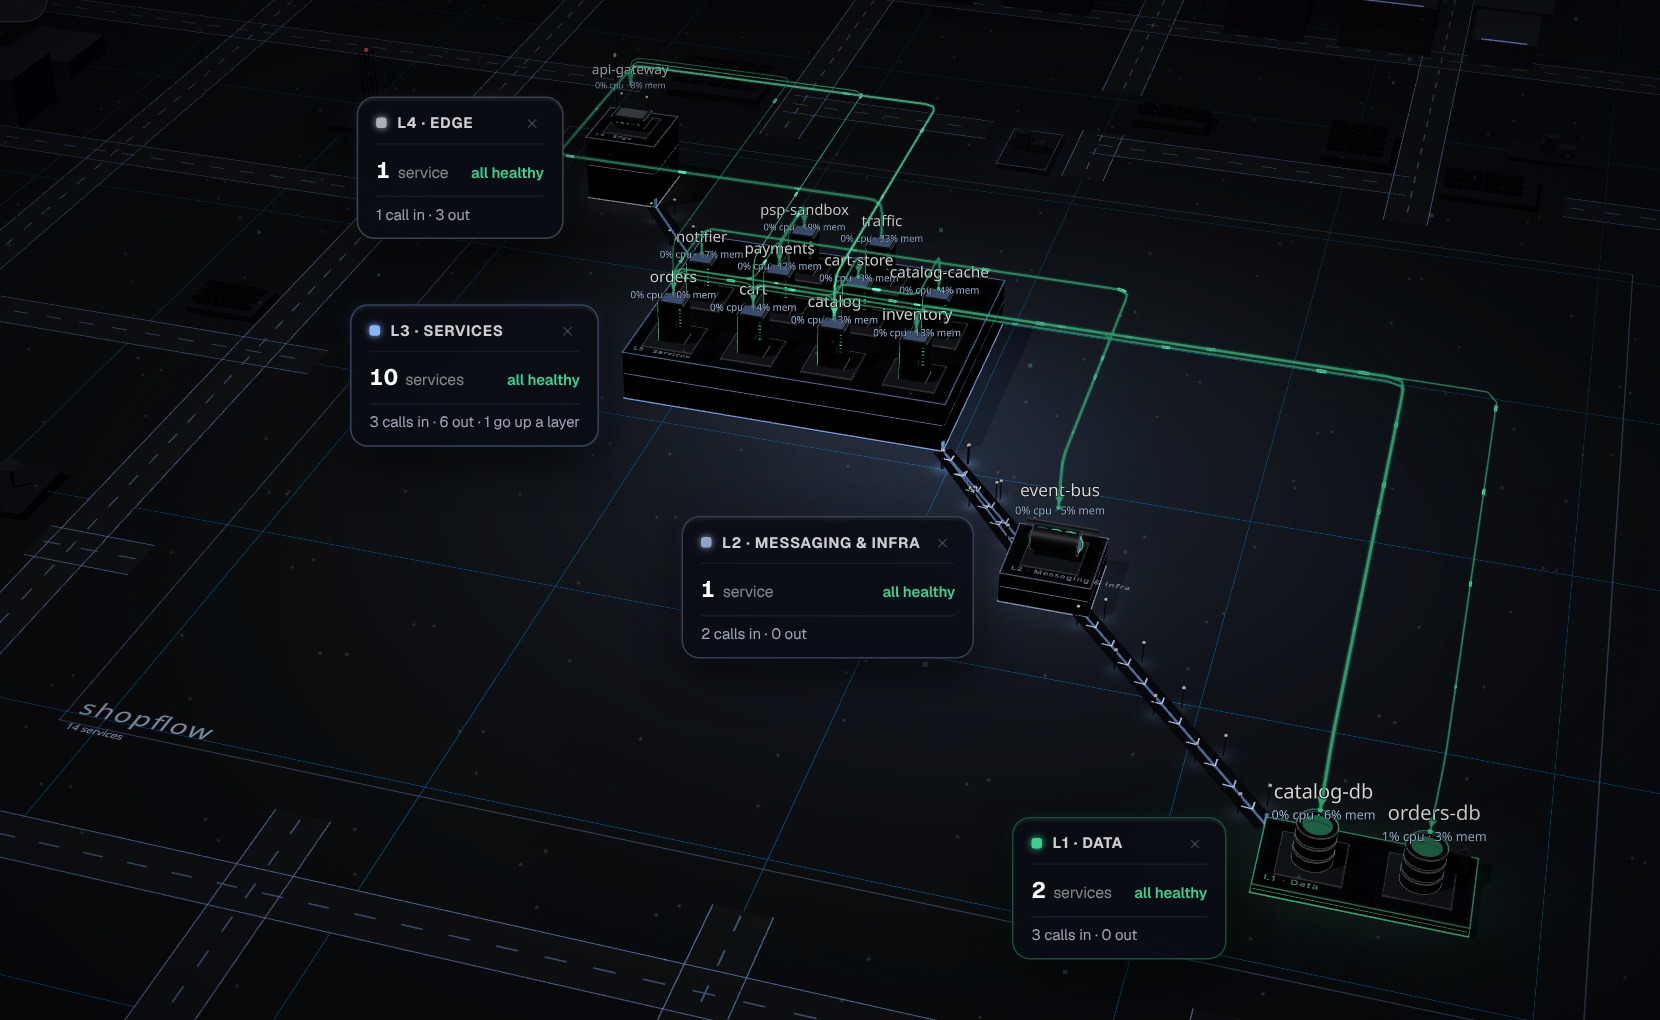
\includegraphics[width=\textwidth]{ui3d_tiers.jpg}\\[-1pt]
{\small (c) Tiers: architectural layers as terraces}
\caption[The Flow, Topology and Tiers arrangements of the 3D view]{The Flow, Topology and Tiers arrangements of the same bench. Each card states what a fault there would mean: how many callers it can reach (Flow), how many services depend on it (Topology), and the calls in and out of each layer (Tiers).}
\label{fig:3d-views}
\end{figure}

\subsection{Research pages}
Three pages that belong to the study rather than daily operation are hidden until the operator switches them on: the ML pipeline (what the hybrid engine sees per service), the model findings of the optional Python sidecar, and the experiment history.

\section{Security Considerations}
\label{sec:security}
The tool holds SSH access to hosts, so it was built to expose as little as it can.
\begin{itemize}
\item \textbf{Keys stay on the operator's machine.} The configuration stores only the path of the key file. Private keys are never copied into the repository, and \texttt{*.pem} files are git-ignored as a backstop.
\item \textbf{A fixed command catalogue.} Every command the server can run on a host is built by a function in one file, and every argument that reaches a shell is checked against the shapes Docker itself produces (container identifiers, timestamps, tail lengths, paths). A test checks that an identifier with shell metacharacters is refused before a command is built.
\item \textbf{Bounded output and time.} Each command has a timeout and a maximum output size, so a misbehaving host cannot make the server wait or buffer without limit.
\item \textbf{Local control surfaces.} The Fault Lab panel listens on localhost only and its requests need a header the page itself sets. Grafana and Prometheus listen on localhost and are reached through an SSH tunnel.
\item \textbf{Ingest token.} The push endpoint is protected by a token. The built-in default is for local use and must be changed when the server can be reached by others.
\item \textbf{One write on the host.} The only change the mapper makes on a host is restarting a container that exited with a non-zero code, a few attempts at most per container, never for load generators, and switched off with \texttt{MAPPER\_AUTO\_RESTART=off}.
\item \textbf{Load limits.} The traffic generator clamps the number of virtual users to a fixed ceiling and starts only from the traffic controller.
\end{itemize}

\section{Testing and Validation}
\label{sec:testing}
The suite has 339 tests in 19 suites and runs in under a minute with \texttt{npm test}. Table~\ref{tab:tests} groups them by area. Three kinds of test deserve a note. \emph{Purity tests} check that algorithm modules do not touch the filesystem or the network, so they can be replayed. \emph{Regression tests} hold each bug that was found (for example the ledger-reader bug and the tier layout). \emph{Security tests} check that the command catalogue refuses unsafe identifiers.

\begin{table}[!htbp]
\centering
\caption{The test suites.}
\label{tab:tests}
\small
\renewcommand{\arraystretch}{1.2}
\begin{tabularx}{\textwidth}{>{\raggedright\arraybackslash}p{5.3cm}>{\raggedright\arraybackslash}X}
\toprule
\textbf{Suite(s)} & \textbf{What is held}\\
\midrule
\texttt{logic}, \texttt{riskEngine}, \texttt{rca} & Layouts (2D and 3D), edge heat scale, risk, cascade, what-if, root-cause scoring\\
\texttt{ml-engine}, \texttt{ml}, \texttt{load-model}, \texttt{rca-research} & Load-aware model (workload invariance, a fault seen during a load change), walk, propagation, hybrid fusion, learned directions, change points\\
\texttt{pipeline}, \texttt{eval}, \texttt{purity} & End-to-end replay, scoring against a ledger, purity of algorithm modules\\
\texttt{telemetry-platform.*} (eight files) & SSH connection, command catalogue, Docker parsers, CPU, units, service identity, storage, discovery, metric collector\\
\texttt{sockets}, \texttt{requestStats}, \texttt{freshness} & Socket direction and recently closed sockets, request statistics, staleness\\
\texttt{security}, \texttt{platform} & Command sanitising, portability across operating systems\\
\texttt{edge-cases}, \texttt{sparse-traffic}, \texttt{target-model} & Missing data, idle services, per-target models\\
\bottomrule
\end{tabularx}
\end{table}

\section{The Two Custom Benchmark Hosts: ShopFlow and LedgerLine}
\label{sec:benches}
The two real systems of the evaluation are not borrowed demos. They were built for this study as \emph{test benches for root-cause-analysis tooling}, each in its own repository and each running on its own EC2 host. The code of both is correct and defensive: every failure comes from configuration, data volume, sizing, topology or a third party, and every failure ships with a machine-readable ground truth (the true root cause, what a monitor should and should not be able to see, and the fix). Each bench has the same four parts: the application, a monitoring stack with Grafana, an always-on traffic generator, and a Fault Lab.

\begin{table}[!htbp]
\centering
\caption{The two benchmark hosts.}
\label{tab:benches}
\small
\renewcommand{\arraystretch}{1.2}
\begin{tabularx}{\textwidth}{>{\raggedright\arraybackslash}p{3.2cm}>{\raggedright\arraybackslash}X>{\raggedright\arraybackslash}X}
\toprule
 & \textbf{ShopFlow} & \textbf{LedgerLine}\\
\midrule
Domain & Online retail checkout & Retail-banking transfers\\
Services & Gateway, catalogue, cart, inventory, payments, orders, an order-event consumer, a third-party payment sandbox; two PostgreSQL, two Redis, NATS (13 services) & Edge, accounts, transfers, fraud screening, FX rates, a double-entry ledger, a statements worker, a third-party FX provider; two PostgreSQL, Redis, NATS (12 services)\\
Public port & 8080 (storefront and API) & 8081 (gateway)\\
Host & EC2 \texttt{c7i-flex.large}, Ubuntu 24.04; about 0.6\,GiB of containers & the same\\
Scenarios with ground truth & 12 (one baseline control) & 7 (one baseline control)\\
Monitoring & Prometheus, Grafana, Loki, Promtail; 25-panel dashboard & the same stack; 25-panel dashboard\\
\bottomrule
\end{tabularx}
\end{table}

\subsection{Monitoring, traffic and the Fault Lab}
Each bench carries a monitoring stack as a \emph{separate Compose project}, so the application project stays exactly what a mapper should discover: Prometheus, Grafana with a provisioned 25-panel dashboard (Figure~\ref{fig:grafana-sf}), Loki with Promtail, and a small exporter that reads per-container CPU, memory, network, restarts and health from the Docker API. Grafana is the operator's ordinary view of a healthy and a faulted bench, and an independent source against which the mapper's readings can be compared on the same time axis. Everything listens on localhost and is reached through an SSH tunnel.

Each bench also has an always-on, open-loop traffic generator. The default mode is \emph{organic}: visitor sessions with think times, popular products, returning users and a day-and-night wave; a steady mode gives a flat load and a quiet mode stops it.

The Fault Lab (\texttt{lab/faultlab} in each bench repository, Figure~\ref{fig:faultlab-sf}) is the fault injector of the evaluation. It is \textbf{blind}: the mapper is never told what is injected, and everything is written to a private ledger read only when scoring. It is \textbf{physical}: faults act on containers (kill, repeated kills, stop, pause, resource limits, network detach, pause-and-release cycles). It is \textbf{organic and reproducible}: a campaign draws faults from a Poisson process with a profile, rate and seed, and the same seed gives the same campaign. Its control page runs on the bench host, listens on localhost only and needs a header the page itself sets, so another site open in the same browser cannot drive it.

\begin{figure}[!htbp]
\centering
\begin{minipage}[b]{0.40\textwidth}\centering
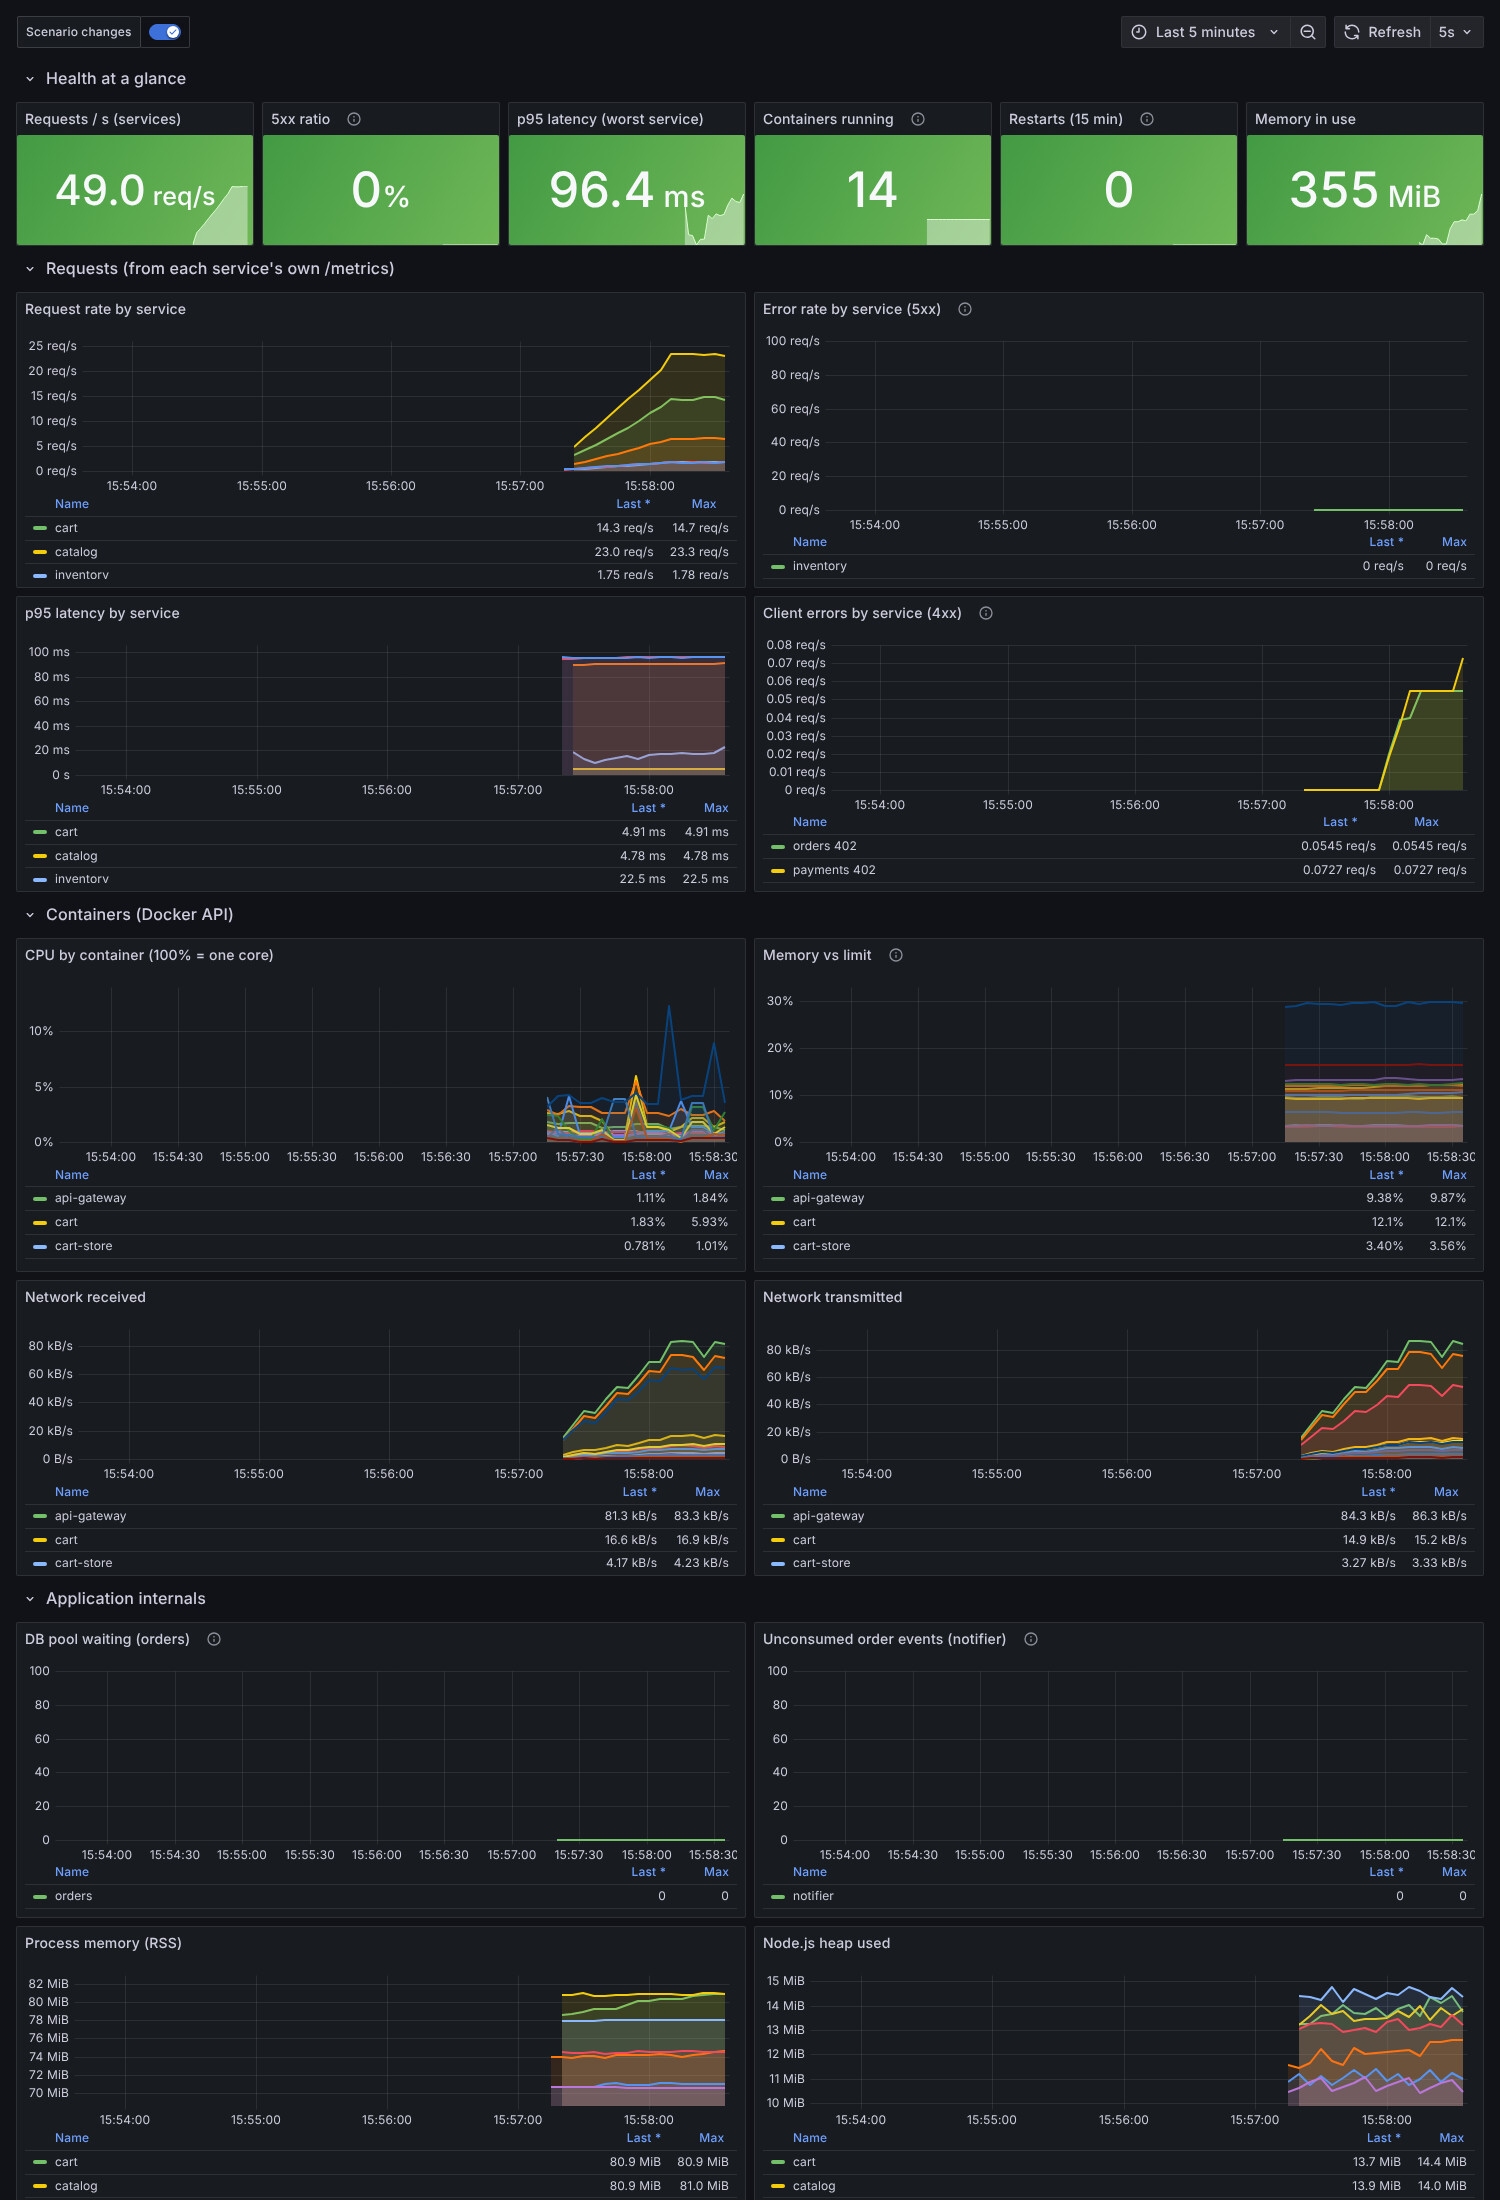
\includegraphics[width=\linewidth]{grafana_shopflow.jpg}
\caption[The provisioned Grafana dashboard of the ShopFlow bench]{The provisioned Grafana dashboard of the ShopFlow bench, from the running bench.}
\label{fig:grafana-sf}
\end{minipage}\hfill
\begin{minipage}[b]{0.56\textwidth}\centering
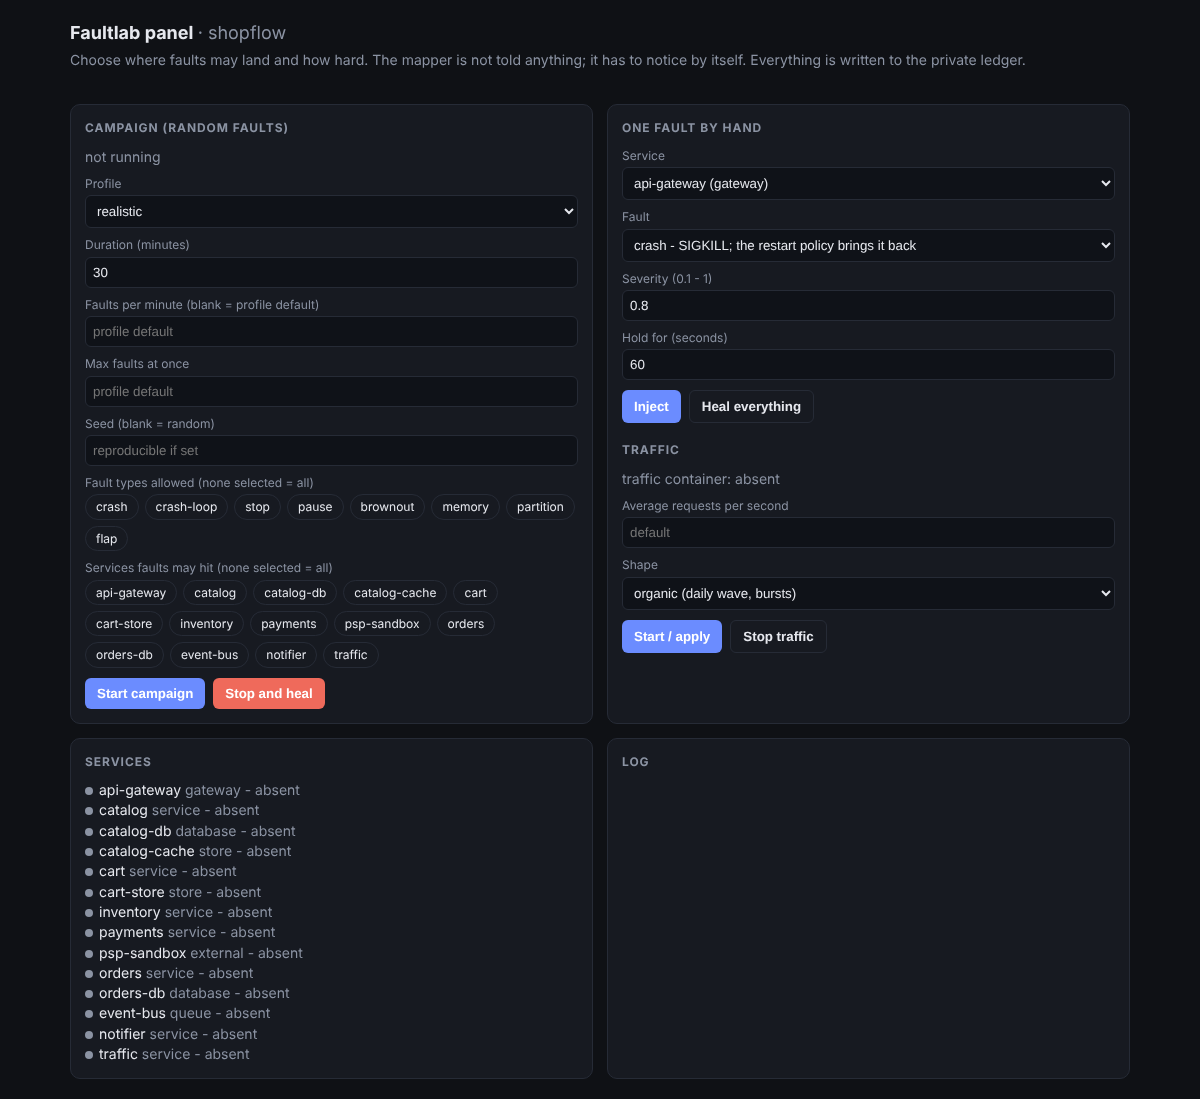
\includegraphics[width=\linewidth]{faultlab_shopflow.png}
\caption[The Fault Lab control page of the ShopFlow bench]{The Fault Lab control page of the ShopFlow bench: a random campaign, one fault by hand, traffic control and the service list.}
\label{fig:faultlab-sf}
\end{minipage}
\end{figure}

\subsection{Scenarios with ground truth}
Besides random campaigns, each bench offers scripted scenarios. A scenario applies a defined cause, drives the load that triggers it, and writes a report beside the expected result stated in its \texttt{scenario.yaml}. Table~\ref{tab:scen-sf} lists those of ShopFlow; LedgerLine has seven more (a pool-starvation cycle between two healthy services, a third-party outage behind a circuit breaker, a hot row, a connection budget, a month-end job that runs out of memory, a shadow dependency, and a baseline). They cover cascades, retry amplification, silent degradation and undocumented dependencies, which are the cases a diagnosis tool most easily gets wrong. The random campaigns of Chapter~\ref{ch:method} are what the reported numbers come from.

\begin{table}[!htbp]
\centering
\caption{ShopFlow scenarios and their true root causes.}
\label{tab:scen-sf}
\footnotesize
\renewcommand{\arraystretch}{1.15}
\begin{tabularx}{\textwidth}{>{\raggedright\arraybackslash}p{3.3cm}>{\raggedright\arraybackslash}X>{\raggedright\arraybackslash}p{2.4cm}}
\toprule
\textbf{Scenario} & \textbf{What happens} & \textbf{Root cause}\\
\midrule
sf-01-missing-index & Order history is fast in staging, melts the database in production & orders-db\\
sf-02-cache-thrash & A cache sized for staging evicts itself in production & catalog-cache\\
sf-03-unbounded-cache & Memory climbs for an hour, then the container is killed & cart\\
sf-04-retry-storm & A third party throttles; our own retries make it ten times worse & psp-sandbox\\
sf-05-secret-rotation & A rotated database password; one service still has the old one & orders\\
sf-06/07 & A dependency that exists only in the code; a declared one nobody calls & none\\
sf-08-noisy-neighbor & A reporting job on the shared database slows checkout & catalog-db\\
sf-09-cpu-throttle & Slow but healthy: a container throttled at a quarter of a core & catalog\\
sf-10-poison-message & One un-processable message stops every confirmation e-mail & notifier\\
sf-11-wrong-hostname & A renamed service still referenced by its old name & none\\
\bottomrule
\end{tabularx}
\end{table}

\section{Host and Mapper Diagnostic Tools}
\label{sec:tools}
Operating the benches showed that ``nothing appears in the dashboard'' has two very different causes: the host cannot answer, or the mapper has a problem. \textbf{\texttt{npm run check-host}} walks one instance step by step and stops at the first failure (port 22, key permissions, login, memory and disk, whether \code{docker} answers within 25 seconds, whether the application answers, which peers each front end calls). \textbf{\texttt{npm run mapper-edges}} prints what the running mapper holds for a project: the target's status, its nodes and every edge with its evidence and last-seen time. Together they separate a host problem from a mapper problem in minutes.

\section{The Evaluation Harness}
\begin{table}[!htbp]
\centering
\caption{The evaluation harness and the experiments built on it.}
\label{tab:harness}
\small
\renewcommand{\arraystretch}{1.2}
\begin{tabularx}{\textwidth}{>{\raggedright\arraybackslash}p{4.4cm}>{\raggedright\arraybackslash}X}
\toprule
\textbf{Command or folder} & \textbf{Purpose}\\
\midrule
\texttt{npm run eval} & Record a fault-injection campaign and score the live mapper (observe, score, report)\\
\texttt{npm run ml:compare} & Compare detectors and root-cause methods on the recorded runs\\
\texttt{npm run ml:hybrid} & Fusion variants of rules and ML\\
\texttt{npm run ml:predict} & Early warning and cascade prediction\\
\texttt{npm run ml:synth} & Synthetic generator (amplification factor, class filter)\\
\texttt{npm run ml:bench} & Cost of one decision window\\
\texttt{v2/} & Studies: learned directions, change-point onset, fault diagnosis\\
\texttt{paper/exp} & Curves, amplification, cascade, router and scaling data for the figures\\
\texttt{run/recorded-runs} & The two recorded runs\\
\bottomrule
\end{tabularx}
\end{table}
